%!TEX root = manual.tex
%===============================================================================
\chapter{Simple housekeeping program}\label{ch:Assignment3}

The aim of this assignment is to experiment with a simple housekeeping program that only implements a basic function, reading a temperature sensor on the on-board computer. The value read by the sensor is denoted as OBC\_T (OBC temperature).
The software is organised in modules, in such a way that it can be later extended to a more complex housekeeping system in the next assignments.

\section{Temperature sensor}

The internal temperature sensor in the MCU is used in this assignment. No additional hardware is required.

The STM32F407 reference manual (section 13.10) states that the internal temperature sensor of the MCU is internally cabled to the {\tt ADC1\_IN16} analog input channel. The steps required to read the sensor are:

\begin{enumerate}
\item Select {\tt ADC1\_IN16} input channel in the ADC.
\item Select a sampling time greater than the minimum sampling time specified in the datasheet (see table~\ref{tb:sensor} below).
\item Set the {\tt TSVREFE} bit in the {\tt ADC\_CCR} register to wake up the temperature sensor from power down mode.
\item Start the ADC conversion by setting the {\tt SWSTART} bit (or by external trigger).
\item Read the resulting VSENSE data in the ADC data register.
\item Calculate the temperature using the following formula:

Temperature (in \degree{C}) = {(VSENSE - V25) / Avg\_Slope} + 25

Where:
\begin{itemize}
\item V25 = VSENSE value for 25 \degree{C} (table~\ref{tb:sensor})
\item Avg\_Slope = average slope of the temperature vs. VSENSE curve (table~\ref{tb:sensor}).
\end{itemize}
\end{enumerate}

The sensor has a startup time after waking from power down mode before it can output VSENSE at the correct level. The ADC also has a startup time after power-on, so to minimize the delay, the {\tt ADON} and {\tt TSVREFE} bits should be set at the same time.

The sensor has a range of -40 to 125 \degree{C}, with a precision of $\pm$1.5 \degree{C}. Its main characteristics are described in the STM32F407 datasheet (table~\ref{tb:sensor}).

\begin{table}[htb]
\begin{center}
\begin{tabular}{llllll} \hline
Symbol & Parameter & Min & Typ & Max & Unit \\ \hline
TL & VSENSE linearity with temperature & - & $\pm1$ & $\pm2$ & \degree{C}\\
Avg\_Slope & Average slope & - & 2.5 & & mV/\degree{C}\\
V25 & Voltage at 25 \degree{C} & - & 0.76 & & V\\
tSTART & Startup time & - & 6 & 10 & $\mu{s}$\\
TS\_temp & ADC sampling time when reading & 10 & - & - & $\mu{s}$\\
& the temperature (1 \degree{C} accuracy) &  &  &  & \\ \hline
\end{tabular}
\caption{STM32F407 temperature sensor characteristic.}
\label{tb:sensor}
\end{center}
\end{table}

The Ada Drivers Library includes the package STM32.ADC, which provides facilities for handling the analog to digital converter.

\section{Software architecture}
The software architecture of the simple housekeeping program is depicted in figure~\ref{fig:simple}\footnote{The graphic notation is AADL (Architecture Analysis and Design Language).}. The software components are:

\begin{figure}[h]
            \centering{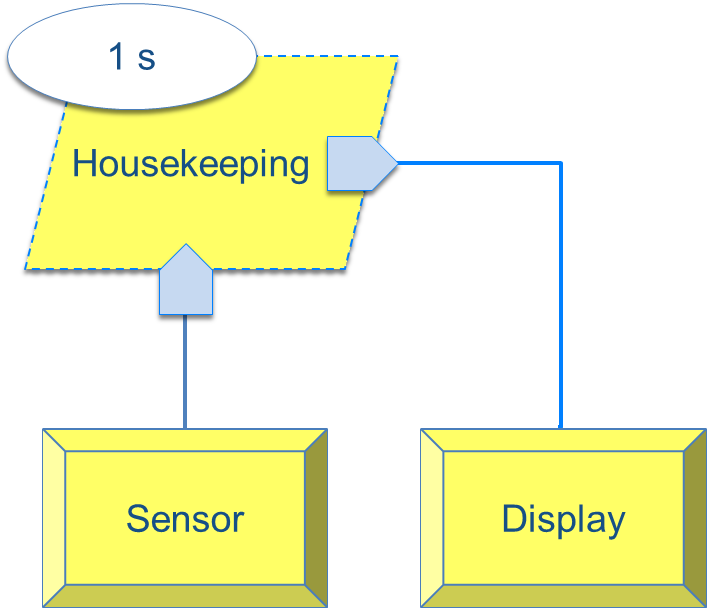
\includegraphics[width=0.5\textwidth,keepaspectratio]{simple.png}}
            \caption{Software architecture of simple housekeeping system.}
            \label{fig:simple}
\end{figure}

\begin{description}
\item[Housekeeping.] Main component, which performs the basic functionality of the system, i.e. reading a temperature value and displaying the value on the console.
\item[Sensor.] This module provides a high-level interface to the temperature sensor and deals with all the details of reading the ADC to which the sensor is connected.
\item[Display.] This module provides a high-level interface to a text console where the measured temperature values can be output.
\end{description}

Since the OBC board does not have a text output device, it has to be simulated on the host computer, using a mechanism called semihosting. When the target board is connected to the host by means of the ST-LINK USB cable, and the embedded program is run using the debugger in the host, the standard output is re-directed to the debugger console. The GPS environment supports semihosting.

\subsection{Download the code and study the implementation}

The implementation code, as initially provided to the students, can be downloaded from \url{https://github.com/STR-UPM/OBDH_LABS}. Click on {\tt Clone} or {\tt download}, download a zip archive, unzip and move to your work directory. The code for this assignment is in the LAB3 folder.

The {\tt Housekeeping} package is the root element of the housekeeping subsystem. Its specification consists of one procedure, {\tt Initialize}, that starts the operation of the component. It has three subpackages:

\begin{description}
\item[Housekeeping.Data] contains the definitions of the data types used in the subsystem. Only one data type, {\tt Analog\_Data}, is defined for this version of the software.

\item[Housekeeping.Sensor] contains the details of the temperature sensor. Its specification includes the {\tt Initialize} and {\tt Get} procedures. This package uses the Ada Drivers Library to interact with the OBC board hardware.

\item[Housekeeping.Display] includes the procedure {\tt Put}, which is used to display temperature values on the debugger console (see below). The original implementation of this procedure writes raw sensor values, which are integers in the range 0 to 4095, as directly provided by the ADC hardware. These values have to be converted to engineering units. i.e. degrees Celsius, using the steps shown in section 3.1 above. The software provided to the students includes a program, {\tt adc2celsius}, which implements this functionality.
\end{description}

The {\tt Display.Put} procedure uses the {\tt Ada.Text\_IO} package to write to the standard output.  Since there is no device that can be used to provide text output on the OBC board, the ST-LINK prove provides a facility, which is called semihosting, to provide this functionality. When the program is run using the cross-debugger on the host, the board standard output is redirected to the debugger console. Therefore, in order to see the temperature values the program must be run from the debugger (see below).

The main procedure is {\tt OBSW}\footnote{On-Board Software}. It calls {\tt Housekeeping.Initialize}, which initializes the sensor and then calls the {\tt Run} procedure. This procedure executes an endless loop that performs the following actions:
\begin{itemize}
\item Get a raw temperature measurement from the sensor
\item Display the value
\end{itemize}

Additionally, one of the board LEDs is toggled on and off to provide a visual check that the program is running.
Notice that {\tt Run}, and hence {\tt Initialize} and {\tt OBSW}, never return. Therefore the program executes indefinitely, as is common in embedded systems.

\section{Compile and run with the debugger.}

Open GPS and do the following:
\begin{enumerate}
\item Select {\tt Open project} on the welcome window. Navigate to the LAB3 directory and open the {\tt simple\_housekeeping.gpr} project file.
\item Build the executable and load it into the board by clicking on the \hbox{
\includegraphics[width=1.5em]{debug.png}} symbol in the tool bar (or select {\tt Build} $\rightarrow$ {\tt Bareboard} $\rightarrow$ {\tt Debug} on board on the top menu).

The program will be compiled, and the executable will be loaded into the board memory by the debugger. After that, the debugger is started\footnote{On Windows a message will be displayed requesting permission to connect st-util to external networks. Be sure to grant such permission to enable the debugger connection to the board.}, and the debugger console (lowest window in GPS) shows the following lines:
\begin{verbatim}
...
(gdb) monitor reset halt
(gdb)
\end{verbatim}

\item Type {\tt continue} or just {\tt c} on the debugger console (or select {\tt Debug} $\rightarrow$ {\tt Continue} on the top menu).
\begin{verbatim}
(gdb) c
Continuing.
[program running]
\end{verbatim}

\item The program will start running (check the LED blinking), and the raw temperature readings are shown on the {\tt Messages} tab of the debugger console (figure~\ref{fig:gdb-output}).
\end{enumerate}

\begin{figure}[h]
            \centering{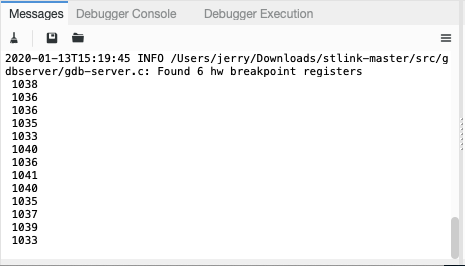
\includegraphics[width=0.8\textwidth,keepaspectratio]{gdb-output.png}}
            \caption{Debugger output.}
            \label{fig:gdb-output}
\end{figure}

The raw measurement values can be converted to Celsius using the {\tt adc2celsius} program. You should take into account that the internal temperature sensor does not provide an accurate measurement, and may have an offset that varies from one chip to another.

\section{Make changes to the program}

As a final activity, you may make some changes to the provided program in order to make sure that you understand the logics behind the source code. Proposed changes are:

\begin{enumerate}
\item Include the conversion to Celsius in the {\tt Display.Put} procedure.
\item Add the following statement to the main loop in the Housekeeping Run procedure:

{\tt delay until Clock + Milliseconds (1000);}

The effect of this statement is to delay the execution of the program for 1 s. You will have to import the {\tt Ada.Real\_Time} library package in order to use the operations included in the statement.
\end{enumerate}
